\documentclass[%handout
,hyperref={pdfpagelabels=false} % beamer hack
,utf8
]{beamer}

\let\Tiny=\tiny % beamer hack

\usepackage{graphicx}
\usepackage{color}
\usepackage{listings}
\usepackage{tikz}
\usetheme{Boadilla}

\setbeamertemplate{footline}%{infolines theme}
{
\leavevmode%
\hbox{%
\begin{beamercolorbox}[wd=.333333\paperwidth,ht=2.25ex,dp=1ex,center]{%
author in head/foot}%
\usebeamerfont{author in head/foot}\insertshortauthor%~~(\insertshortinstitute)
\end{beamercolorbox}%
\begin{beamercolorbox}[wd=.333333\paperwidth,ht=2.25ex,dp=1ex,center]{%
title in head/foot}%
\usebeamerfont{title in head/foot}\insertshorttitle
\end{beamercolorbox}%
\begin{beamercolorbox}[wd=.333333\paperwidth,ht=2.25ex,dp=1ex,right]{%
date in head/foot}%
\usebeamerfont{date in head/foot}\insertshortdate{}\hspace*{2em}
\insertframenumber{} / \inserttotalframenumber\hspace*{2ex}
\end{beamercolorbox}}%
\vskip0pt%
}

\mode<all>
{
\newenvironment<>{curryblock}[1]{%
    \begin{actionenv}#2%
      \def\insertblocktitle{#1}%
      \par%
      \setbeamercolor{block title}{fg=orange, bg=orange!30}%
      \usebeamertemplate{block begin}}
    {\par%
      \usebeamertemplate{block end}%
    \end{actionenv}}
}

\newenvironment{program}{\begin{semiverbatim}\small}{\end{semiverbatim}}
\newcommand{\code}[1]{\texttt{#1}}
\newcommand{\todo}[1]{\fbox{\sc To do: #1}}

%%%%%%%%%%%%%%%%%%%%%%%%%%%%%%%%%%%%%%%%%%%%%%%%%%%%%%%%%%%%%%%%%%%%%%%%%%%%%%%%

\begin{document}

\title[KiCS2]{KiCS2: A New Compiler from Curry to Haskell}

\date[WFLP 2011]{WFLP 2011, July 19}

\author[B. Braßel, M. Hanus, \underline{B. Peemöller}, F. Reck]{%
Bernd Braßel \and Michael Hanus \\
\underline{Björn Peemöller} \and Fabian Reck\\
\texttt{\{bbr, mh, bjp, fre\}@informatik.uni-kiel.de}
}

\institute{Kiel University}

\begin{frame}%---------------
\titlepage
\end{frame}

%%%%%%%%%%%%%%%%%%%%%%%%%%%%%%%%%%%%%%%%%%%%%%%%%%%%%%%%%%%%%%%%%%%%%%%%%%%%%%%%

\section{Introduction}

\begin{frame}[fragile]%---------------------------------------------------------
\frametitle{Curry}
\begin{columns}[t]
\column{.45\textwidth}
\begin{itemize}
\item Lazy functional logic programming language
\item Haskell-like syntax
\item Extended by non-determinism, free variables, constraints, unification
\end{itemize}

\begin{example}<2>
\begin{program}
> xorSelf aBool
False
\textsl{More solutions?} y
False
\end{program}
\end{example}

\column{.45\textwidth}
\begin{curryblock}{Running Code Snippet}
\begin{program}
data Bool = True | False

aBool :: Bool
aBool = True ? False

not True  = False
not False = True

xor True  x = not x
xor False x = x

xorSelf x = xor x x
\end{program}
\end{curryblock}
\end{columns}
\end{frame}


\begin{frame}%------------------------------------------------------------------
\frametitle{KiCS2}
% \begin{block}{Previous implementation approaches}
% \begin{itemize}
%  \item Compile to abstract machine (MCC compiles to C)
%  \item Compile to logic language (PAKCS compiles to Prolog)
%  \item Compile to functional language (KiCS compiles to Haskell)
% \end{itemize}
% \end{block}
% \pause

\begin{block}{Our Approach}
\begin{itemize}
\item Compile Curry programs into Haskell programs
\item Reuse features of Haskell 
      (lazy evaluation, higher-order functions)
\item Benefit from mature Haskell compiler (GHC)
%      and its future improvements
\end{itemize}
\end{block}
\pause

\begin{block}{Goals}
\begin{itemize}
\item Efficiently execute purely functional programs
\item Avoid unsafe operations to enable optimization 
      (in contrast to KiCS)
\item Support different search strategies 
      (including complete strategies)
\end{itemize}
\end{block}

\end{frame}

%%%%%%%%%%%%%%%%%%%%%%%%%%%%%%%%%%%%%%%%%%%%%%%%%%%%%%%%%%%%%%%%%%%%%%%%%%%%%%%%

\section{Compilation scheme}

\begin{frame}[fragile]%---------------------------------------------------------
\frametitle{Representation of Non-Determinism}
\begin{itemize}
  \item No built-in non-determinism in Haskell
  \item Idea: Explicit representation in data types as constructors
\end{itemize}
\pause

\begin{curryblock}{Curry}
\begin{program}
data Bool = True | False

aBool :: Bool
aBool = True ? False
\end{program}
\end{curryblock}

\begin{block}{Haskell}
\begin{program}
data Bool = True | False | Choice Bool Bool

aBool :: Bool
aBool = Choice True False
\end{program}
\end{block}
\end{frame}


\begin{frame}[fragile]%---------------------------------------------------------
\frametitle{Extension of Operations}
\begin{itemize}
  \item Operations have to deal with non-deterministic values
  \item Pattern matching is extended
  \item Non-determinism in arguments is propagated
\end{itemize}
\pause

\begin{block}{Haskell}
\begin{program}
not True             = False
not False            = True
not (Choice x1 x2)   = Choice (not x1) (not x2)

xor True           x = not x
xor False          x = x
xor (Choice x1 x2) x = Choice (xor x1 x) (xor x2 x)

xorSelf x            = xor x x
\end{program}
\end{block}
\end{frame}


\begin{frame}[fragile]%---------------------------------------------------------
\frametitle{Evaluation with non-deterministic arguments}
\begin{exampleblock}{Evaluation without sharing}
\code{not aBool}\\
$\leadsto$ \code{not (Choice True False)}\\
$\leadsto$ \code{Choice (not True) (not False)}\\
$\leadsto$ \code{Choice False True}
\end{exampleblock}
\pause

\begin{exampleblock}{Evaluation with sharing}
\code{xorSelf aBool}\\
$\leadsto$ \code{xor aBool aBool}\\
$\leadsto$ \code{xor (Choice True False) aBool}\\
$\leadsto$ \code{Choice (xor True aBool) (xor False aBool)}\\
$\leadsto$ \code{Choice (not aBool) aBool}\\
$\leadsto$ \code{Choice (Choice False True) (Choice True False)}
\end{exampleblock}

\begin{itemize}
  \item Yields two results \code{True} and \code{False}
  \item Only \code{False} is correct w.r.t. the semantics of Curry
\end{itemize}
\end{frame}


\begin{frame}[fragile]%---------------------------------------------------------
\frametitle{Call-Time Choice vs. Run-Time Choice}
\begin{curryblock}{Curry}
\begin{program}
xorSelf x = xor x x
\end{program}
\end{curryblock}
\pause

\begin{block}{Call-Time Choice}
\begin{itemize}
\item Variables denote values
\item Both occurrences of \code{x} are substituted with the same value 
      in each non-deterministic branch
\end{itemize}
\end{block}
\pause

\begin{block}{Run-Time Choice}
\begin{itemize}
\item Variables denote non-deterministic computations
\item Substitutions of \code{x} may evaluate to different values 
      in the same non-deterministic branch
\end{itemize}
\end{block}
\pause

\begin{itemize}
\item Call-Time Choice is often more intuitive
\item Curry has Call-Time Choice semantics 
\item Unrestricted propagation violates Call-Time Choice
\end{itemize}
\end{frame}


\begin{frame}[fragile]%---------------------------------------------------------
\frametitle{Identifying Choices}
To preserve call-time choice semantics
\begin{itemize}
\item Choices are annotated with unique identifiers
\item Decisions made for different occurrences of the same choice
      have to be consistent
\end{itemize}
\pause

\begin{block}{Choice Identifier}
\begin{program}
\alert{type ID = Integer}

data Bool = False | True | Choice \alert{ID} Bool Bool

not (Choice \alert{i} x1 x2) = Choice \alert{i} (not x1) (not x2)

xor (Choice \alert{i} x1 x2) x = Choice \alert{i} (xor x1 x) (xor x2 x)
\end{program}
\end{block}
\end{frame}


\begin{frame}[fragile]%--------------------------------------------------------
\frametitle{Choice Identifiers}
\begin{itemize}
 \item \code{ID}s are provided by an \code{IDSupply} (infinite set of \code{ID}s)
 \item \code{IDSupply}s can be split into disjoint subsets
 \item Functions that may introduce non-determinism
       are provided with an \code{IDSupply}
\end{itemize}

\pause

\begin{block}{Choice Identifier}
\begin{program}
type IDSupply = Integer

thisID :: IDSupply -> ID
thisID n = n

aBool :: \alert{IDSupply ->} Bool
aBool \alert{s} = Choice \alert{(thisID s)} True False
\end{program}
\end{block}
\end{frame}


\begin{frame}[fragile]%--------------------------------------------------------
\frametitle{Evaluation revisited}

\begin{exampleblock}{Evaluation with sharing}
\code{xorSelf (aBool 1)}\\
$\leadsto$ \code{xor (aBool 1) (aBool 1)}\\
$\leadsto$ \code{xor (Choice 1 True False) (Choice 1 True False)}\\
$\leadsto$ $\dots$\\
$\leadsto$ \code{Choice 1 (Choice 1 False True) (Choice 1 True False)}
\end{exampleblock}

\begin{center}
\begin{tikzpicture}
\node (a) at (0,0) {\code{True}};
\node (b) at (2,0) {\code{False}};
\node (c) at (0,1.5) {$\code{?}_{1}$};
\node (d) at (2,1.5) {$\code{?}_{1}$};
\node (e) at (1,2) {$\code{?}_{1}$};
\draw (e) -- (c);
\draw (e) -- (d);
\draw (c.south west) .. controls (0,0) and (1,2) .. (b);
\draw[style=dashed] (c.south east) -- (a);
\draw[style=dashed] (d.south west) -- (a);
\draw (d.south east) -- (b);
\end{tikzpicture}
\end{center}
Only \code{False} ist reachable with consistent decisions
\end{frame}


% \begin{frame}[fragile]%--------------------------------------------------------
% \frametitle{Representing Failure}
% \begin{itemize}
%  \item Computing with failure is a common programming pattern in FLP
%  \item Failures do not abort the computation, but are ignored
%  \item Thus, failures have to be represented as well
% \end{itemize}
% \begin{curryblock}{Curry}
% \begin{program}
% data Bool = True | False
% 
% ensureTrue True = True
% \end{program}
% \end{block}
% \begin{block}{Haskell}
% \begin{program}
% data Bool = True | False | Choice ID Bool Bool | Fail
% 
% ensureTrue True             = True
% ensureTrue (Choice i x1 x2) = Choice i (ensureTrue x1) ensureTrue (x2)
% ensureTrue _                = Fail
% \end{program}
% \end{curryblock}
% \end{frame}


\begin{frame}[fragile]%---------------------------------------------------------
\frametitle{Higher-Order Functions}
\begin{itemize}
\item Non-deterministic functions need an \code{IDSupply}
      as an additional parameter
\item In higher-order functions, the supply is passed 
      to the functional argument when applied
\end{itemize}
\pause

\vspace{-2ex}

\begin{columns}[t]
\column{.45\textwidth}
\begin{curryblock}{Curry}
\begin{program}
apply :: (a -> b) 
      ->  a -> b
apply f x = f x

func b = b ? not b

> apply func True
True
False
\end{program}
\end{curryblock}

\column{.45\textwidth}
\begin{block}{Haskell}
\begin{program}
apply :: (a -> IDSupply -> b) 
      ->  a -> IDSupply -> b
apply f x s = f x s

func b s = Choice (thisID s) 
           b (not b)

> apply func True 1
Choice 1 True False
\end{program}
\end{block}
\end{columns}
\end{frame}


\begin{frame}[fragile]%---------------------------------------------------------
\frametitle{Higher-Order Optimization}
\begin{itemize}
  \item To be used in higher-order functions, 
        deterministic functions have to be wrapped

\vspace{-2ex}
\begin{columns}[t]
\column{.45\textwidth}
\begin{curryblock}{Curry}
\begin{program}
> apply not True
False
\end{program}
\end{curryblock}
\column{.45\textwidth}
\begin{block}{Haskell}
\begin{program}
> apply (\\x _ -> not x) True 1
False
\end{program}
\end{block}
\end{columns}
\vspace{2ex}
\pause

\item To avoid overhead, higher-order functions are translated into
  \begin{itemize}
   \item a deterministic variant
   \item a non-deterministic variant
  \end{itemize}
\item Deterministic functions only call deterministic variants
\item Benchmarks show enormously improved performance
\end{itemize}
\end{frame}

%%%%%%%%%%%%%%%%%%%%%%%%%%%%%%%%%%%%%%%%%%%%%%%%%%%%%%%%%%%%%%%%%%%%%%%%%%%%%%%%

\section{Benchmarks}

\begin{frame}%------------------------------------------------------------------
\frametitle{Benchmark: Deterministic First-Order Function}
\begin{itemize}
\item Program: naive reverse of a user-defined list structure
\item Functional programs run with almost no overhead
\end{itemize}
\begin{center}
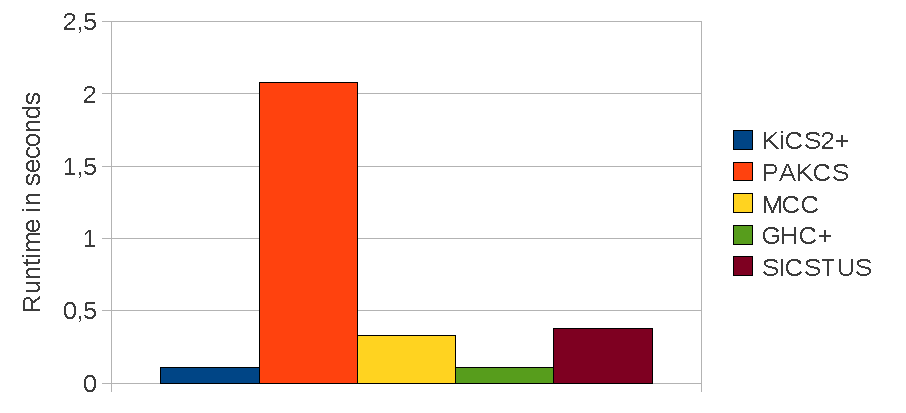
\includegraphics[width=11cm]{gfx/reverse}
\end{center}
\end{frame}

\begin{frame}%------------------------------------------------------------------
\frametitle{Benchmark: Deterministic Higher-Order Function}
\begin{itemize}
\item Program: reverse of a user-defined list using foldl
\item Higher-order optimization dramatically improves performance
\end{itemize}
\begin{center}
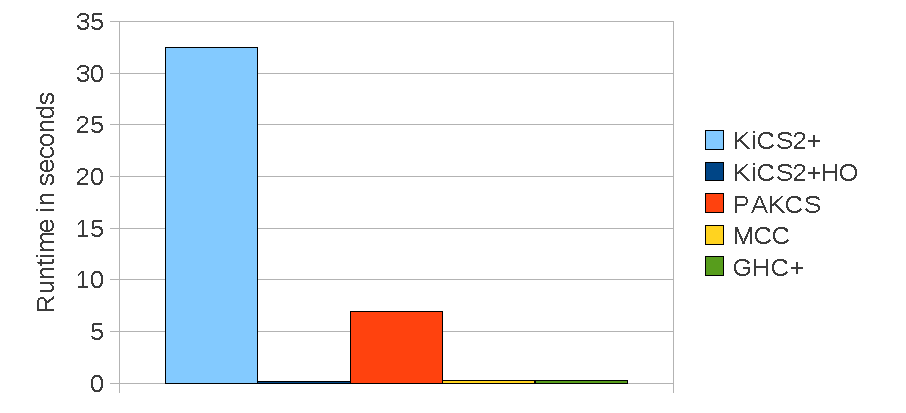
\includegraphics[width=11cm]{gfx/reverseho}
\end{center}
\end{frame}

\begin{frame}%------------------------------------------------------------------
\frametitle{Benchmark: Non-Deterministic Permutation Sort}
\begin{itemize}
\item Program: permutation sort
\item KiCS2 can compete with existing compilers
\end{itemize}
\begin{center}
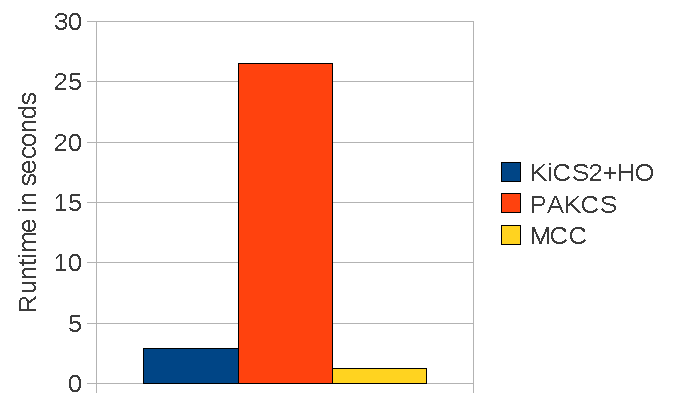
\includegraphics[width=11cm]{gfx/permsort}
\end{center}
\end{frame}

\begin{frame}[fragile]%---------------------------------------------------------
\frametitle{Benchmark: Halve a Peano Number}
\begin{itemize}
\item Program: halve a Peano number by inverting addition
\item There is still much room for improvements
\end{itemize}
\begin{center}
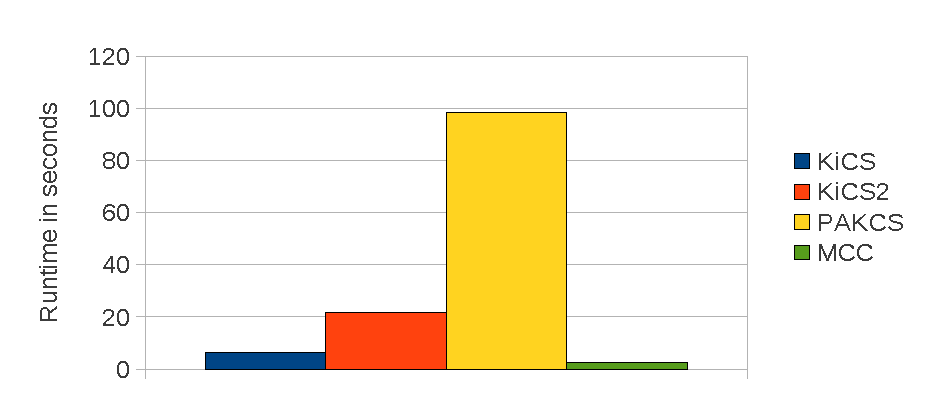
\includegraphics[width=11cm]{gfx/half}
\end{center}
\end{frame}

%%%%%%%%%%%%%%%%%%%%%%%%%%%%%%%%%%%%%%%%%%%%%%%%%%%%%%%%%%%%%%%%%%%%%%%%%%%%%%%%

\section{Conclusion}

\begin{frame}%------------------------------------------------------------------
\frametitle{Status quo}
\begin{itemize}
\item Additional Features (work in progress)
      \begin{itemize}
      \item Free (logic) variables and unification
      \item Functional patterns
      \item Sharing over non-determinism
      \item Different search strategies 
            (depth-first, breadth-first, iterative deepening, parallel)
      \item Encapsulated search
      \end{itemize}
\item Future work
      \begin{itemize}
      \item More detailed analysis to decrease overhead of logic features
      \item Implementation of set functions
      \item First release (coming soon)
      \end{itemize}
\end{itemize}
\end{frame}


\begin{frame}%------------------------------------------------------------------
\frametitle{Conclusion}
\begin{itemize}
\item Transformation of a functional logic program into a functional program
\item Resulting program can be optimized by the Haskell compiler
\item Our approach can compete with or outperform existing implementations
\item A formal description of our approach can be found in our paper
\end{itemize}
\end{frame}

\end{document}
